\documentclass[class=article, crop=false, dvipdfmx, fleqn]{standalone}
\title{航空機設計法第一 \\
レポート課題3 \ 機体三面図(初期案)}
\author{学籍番号 03-170313 飯山 敬大\\
        }
\date{\today}

% packages and libraries
\usepackage[utf8]{inputenc}				%fonts
\usepackage[ipaex]{pxchfon}
\usepackage{pifont}
\usepackage{mathtools, amssymb, mathrsfs, bbm,nccmath}	%math
\usepackage{siunitx, physics}
\usepackage[table]{xcolor}				%colors
\usepackage{tabularx}
\usepackage[dvipdfmx]{graphicx}					%figures
\usepackage{subcaption, wrapfig}
\usepackage{tikz}
\usetikzlibrary{calc, patterns, decorations, angles, calendar, backgrounds, shadows, mindmap}
\usepackage{tcolorbox}					%tables
\usepackage{longtable, float, multirow, array, listliketab, enumitem, tabularx}
\usepackage{listings}					%listings
\usepackage{comment}
\usepackage{hyperref}					%URL, link
\usepackage{url}
\usepackage{pxjahyper}
\usepackage{overcite}					%setting of citation
\usepackage{pxrubrica}					%rubi
\usepackage{fancyhdr, lastpage}			%pagelayout
\usepackage{import, grffile}			%file management
\usepackage{standalone}
\usepackage{bm}
\usepackage{empheq}
\usepackage{pdfpages}
\usepackage{multicol}
% set up for siunitx
\sisetup{%
	%detect-family = true,
	detect-inline-family = math,
	detect-weight = true,
	detect-inline-weight = math,
    %input-product = *,
    quotient-mode = fraction,
	fraction-function = \frac,
	inter-unit-product = \ensuremath{\hspace{-1.5pt}\cdot\hspace{-1.5pt}},
	per-mode = symbol,
	product-units = single,
	}

% setting of line skip
\setlength{\lineskiplimit}{6pt}
\setlength{\lineskip}{6pt}

% setting of indent
\setlength{\parindent}{1zw}
\setlength{\mathindent}{5zw}

% change cite form
\renewcommand{\citeform}[1]{[#1]}

% number equations only when they are referred to in the text
\mathtoolsset{showonlyrefs=true}
%\graphicspath{{images/}{../images/}}

% set up for hyperref
\hypersetup{%
	bookmarksnumbered = true,%
	hidelinks,%
	colorlinks = true,%
	linkcolor = black,%
	urlcolor = cyan,%
	citecolor = black,%
	filecolor = magenta,%
	setpagesize = false,%
	}

\pdfstringdefDisableCommands{%
\renewcommand*{\bm}[1]{#1}%
% any other necessary redefinitions
}
% Include \subsubsection in ToC
\setcounter{tocdepth}{3}

% tabularx
\newcolumntype{C}{>{\centering\arraybackslash}X} %セル内で中央揃え
\newcolumntype{R}{>{\raggedright\arraybackslash}X} %セル内で右揃え
\newcolumntype{L}{>{\raggedleft\arraybackslash}X}

\begin{document}
\section{カルマンフィルターの作成}
$\bm{q},\bm{\omega}$の真値は式(6)を課題1で議論した方法により数値積分することで求めることができる.
ここでは, 状態方程式(8)を離散化して, 離散化カルマンフィルタを組むことによって真値からのずれ$\bm{x}$
を推定することを考える.
状態k-1からkへの遷移が, 次の線形の推移行列
\begin{equation}
  \dot{\bm{x_k}} = \bm{\Phi_{k-1}}\bm{x_{k-1}} + \Gamma_{k-1}w_{k-1}
\end{equation}
で与えられるとすると, 式(8)より
\begin{align}
  & \bm{\phi_{k}} = e^{\bm{A}(t)\Delta t} \\
  & \bm{\Gamma_{k}} = \bm{A(t)}^{-1}(e^{\bm{A}(t)\Delta t} - \bm{I})\bm{B}(t)
\end{align}
となる. 離散カルマンフィルタのアルゴリズムは,以下のようになる.
ただし,
\begin{enumerate}
  \item $\overline{\bm{x_k}}$ : 観測を行う前の真値からのずれ$\bm{x_k}$の推定値
  \item $\hat{\bm{x_k}}$ : 観測を行った後の真値からのずれ$\bm{x_k}$の推定値
  \item $\bm{M_k}$ : 観測を行う前の推定誤差の共分散($\bm{P_{k-1}}$と状態方程式による推定)
  \item $\bm{P_k}$ : 観測を行った後の推定誤差の共分散
\end{enumerate}
とする.
\begin{enumerate}
  \item 真値は課題1のシミュレータに, 外乱トルクw(乱数を使ってホワイトノイズとして作成)
  を加えて(6)式を時間積分して作成する.
  \item 状態遷移時の更新(0.01秒おき): システム推定値は, 最初適当な初期値を乱数で発生させ, (6)式を$\bm{w}$=0で時間積分することで
  求める. また, $\bm{M_k}$と$\bm{P_k}$を
  \begin{align}
    &\bm{M_k} = \bm{\Phi_{k-1}} \bm{P_{k-1}} {\bm{\Phi_{k-1}}}^{\mathrm{T}} +
    \bm{\Gamma_{k-1}} \bm{Q_{k-1}} {\bm{\Gamma_{k-1}}}^{\mathrm{T}} \\
    &\bm{P_k} = \bm{M_k}
  \end{align}
  によって更新していく. 観測を行っていないので, 観測による補正は行っていない(第二式)ことに注意する.
  \item 観測時の更新(0.1秒おき): 真値からのずれ$\bm{x}$は実際には計算できないので、観測方程式(式(15))から$\bm{z}$を計算
  することはできない. よって観測によって得られる$\bm{y}$と推定系より得られる$\hat{\bm{y}}$(推定系では
  $\bm{v}$=0)から,
  \begin{equation}
    \bm{z_k} = \bm{y_k} - \hat{\bm{y_k}}
  \end{equation}
  と計算する. 推定誤差の共分散Pは
  \begin{equation}
    \bm{P_k} = \bm{M_k} - \bm{M_k}{\bm{H_k}}^{\mathrm{T}}{(\bm{H_k}\bm{M_k}{\bm{H_k}}^{\mathrm{T}} + \bm{R_k})}^{-1}
    \bm{H_k}\bm{M_k}
  \end{equation}
  と更新され, カルマンゲイン$\bm{K_k}$を
  \begin{equation}
    \bm{K_k} = \bm{P_k}{\bm{H_k}}^{\mathrm{T}}{\bm{R_k}}^{-1}
  \end{equation}
  と計算する.
  \item 観測を行った後の$\bm{x_k}$の推定値は,
  \begin{equation}
    \hat{\bm{x_k}} = \bm{K_k}\bm{z}
  \end{equation}
  と推定される. 推定系
  $
  {\begin{bmatrix}
    \bm{q} \\
    \bm{\omega}
  \end{bmatrix}}_k
  $は,
  \begin{equation}
    {\begin{bmatrix}
      \bm{q} \\
      \bm{\omega}
    \end{bmatrix}}_k =
    {\begin{bmatrix}
      \bm{q} \\
      \bm{\omega}
    \end{bmatrix}}_k + \hat{\bm{x_k}}
  \end{equation}
  と更新される. また更新時にQuartanionのノルムを保存するため, 正規化する. \\
  以上で述べたカルマンフィルターの構成を図にすると,図1のようになる. またカルマンフィルターを
  含めたシステム全体のブロック線図は, 図2のようになる.

  \begin{figure}[H]
    \begin{center}
    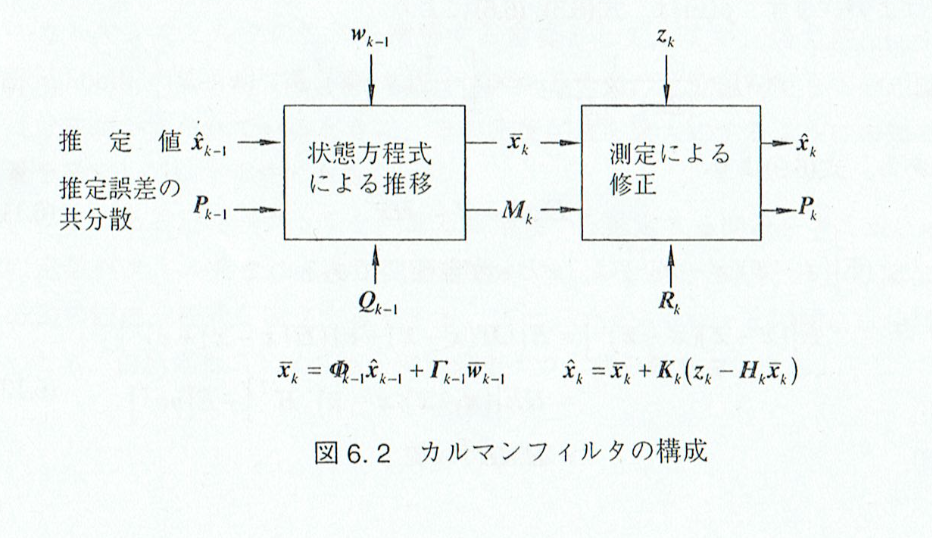
\includegraphics[width=8cm]{../images/kalman_system.png}
    \caption{カルマンフィルタの構成}
    \label{kalman_system}
  \end{center}
  \end{figure}

  \begin{figure}[H]
    \begin{center}
    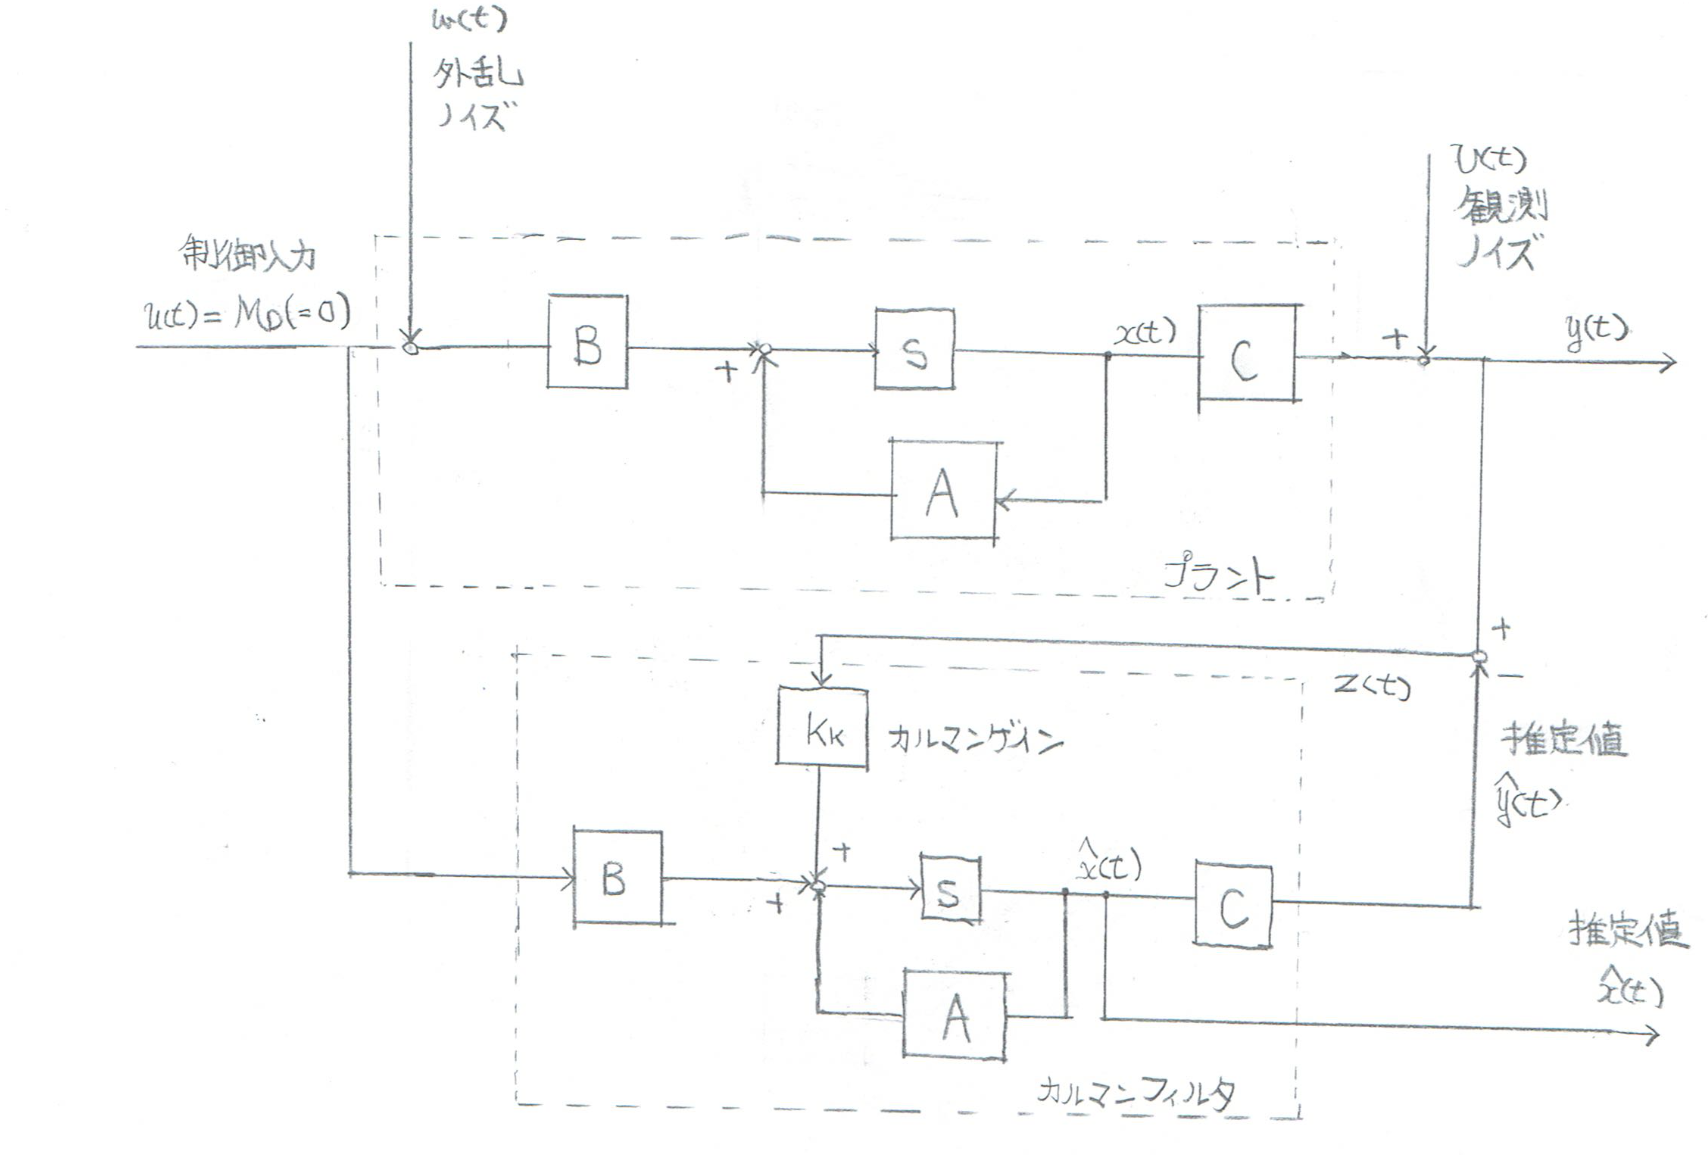
\includegraphics[width=8cm]{../images/kalman_block.png}
    \caption{ブロック線図}
    \label{kalman_block}
  \end{center}
  \end{figure}

\end{enumerate}
\end{document}
